../../hw03/report/pcsmacros.tex
\include{pythonlisting}
\def\xs{{\xx_s}}


\title[]{Extended imaging and tomography under two-way operators}
\subtitle{}
\author[]{Esteban D\'{i}az}
\date{}
\logo{}



\huge

\def\big#1{\begin{center} \LARGE \textbf{#1} \end{center}}
\def\cen#1{\begin{center}        \textbf{#1} \end{center}}


\tikzstyle{arrow}=[draw, -latex] 
\tikzstyle{rarrow}=[arrow,line width=.8mm,draw=red, fill=red]
\tikzstyle{karrow}=[arrow,scale=.5,line width=.8mm,draw=black, fill=black]
\tikzstyle{RectObject}=[rectangle,fill=white,draw,line width=0.5mm]


% ------------------------------------------------------------
\mode<beamer> { \cwpcover }

%\setbeamertemplate{footline}[frame number] 



\inputdir{XFig}


\begin{frame}
\vspace{-2cm}
  \plot{objectiveFWD}{width=\textwidth}{}
\end{frame}
\begin{frame}
\vspace{-2cm}
  \plot{objectiveSCT}{width=\textwidth}{}
\end{frame}


\begin{frame}
\vspace{-2cm}
  \plot{swfl}{width=\textwidth}{}
\end{frame}



\begin{frame}
\vspace{-2cm}
  \plot{rwfl}{width=\textwidth}{}
\end{frame}

\begin{frame}
\vspace{-2cm}
  \plot{objectiveIMG}{width=\textwidth}{}
\end{frame}


\begin{frame}
\vspace{-2cm}
  \plot{SCT}{width=\textwidth}{}
\end{frame}




\begin{frame}
\vspace{-2cm}
  \plot{objectiveTOM}{width=\textwidth}{}
\end{frame}




\begin{frame} \frametitle{previous projects}
  \large
  \begin{enumerate}
    \item {\bf E. D\'{i}az} and P. Sava. Understanding rtm backscattering: noise or signal?. Geophysical Prospecting, 64: 581–594 (2015).
    \item {\bf E. D\'{i}az} and P. Sava. Wavefield tomography using rtm backscattering. Geophysics 80.1 (2014): R57-R69.
    \item {\bf E. D\'{i}az}, P. Sava , and T. Yang. "Data-domain and image-domain wavefield tomography”. The Leading Edge 2013 32:9, 1064-1072 
    \item  Kamath, N., Tsvankin, I., and {\bf D\'{i}az, E}. "Elastic FWI for VTI media: A synthetic parameterization study”. Geophysics (2017, submitted). 
    \item Pedrassi, M., Behura, J., Davis, T. L.,  {\bf D\'{i}az, E.}, \& Singh, S. (2015). Application of waveform tomography at the Campos Basin field. First Break, 33(9), 87-93
  \end{enumerate} 
\end{frame}


\begin{frame} \frametitle{previous projects}
  \large
  \begin{enumerate}
    \item {\bf E. D\'{i}az} and P. Sava. Understanding rtm backscattering: noise or signal?. Geophysical Prospecting, 64: 581–594 (2015).
    \item {\bf E. D\'{i}az} and P. Sava. Wavefield tomography using rtm backscattering. Geophysics 80.1 (2014): R57-R69.
    \item \gray{{\bf E. D\'{i}az}, P. Sava , and T. Yang. "Data-domain and image-domain wavefield tomography”. The Leading Edge 2013 32:9, 1064-1072 }
    \item \gray{ Kamath, N., Tsvankin, I., and {\bf D\'{i}az, E}. "Elastic FWI for VTI media: A synthetic parameterization study”. Geophysics (2017, submitted).} 
    \item \gray{Pedrassi, M., Behura, J., Davis, T. L.,  {\bf D\'{i}az, E.}, \& Singh, S. (2015). Application of waveform tomography at the Campos Basin field. First Break, 33(9), 87-93}
  \end{enumerate} 
\end{frame}


\begin{frame} \frametitle{previous projects}
  \large
  \begin{enumerate}
    \item \gray{{\bf E. D\'{i}az} and P. Sava. Understanding rtm backscattering: noise or signal?. Geophysical Prospecting, 64: 581–594 (2015).}
    \item \gray{{\bf E. D\'{i}az} and P. Sava. Wavefield tomography using rtm backscattering. Geophysics 80.1 (2014): R57-R69.}
    \item {\bf E. D\'{i}az}, P. Sava , and T. Yang. "Data-domain and image-domain wavefield tomography”. The Leading Edge 2013 32:9, 1064-1072 
    \item  \gray{Kamath, N., Tsvankin, I., and {\bf D\'{i}az, E}. "Elastic FWI for VTI media: A synthetic parameterization study”. Geophysics (2017, submitted).} 
    \item \gray{Pedrassi, M., Behura, J., Davis, T. L.,  {\bf D\'{i}az, E.}, \& Singh, S. (2015). Application of waveform tomography at the Campos Basin field. First Break, 33(9), 87-93}
  \end{enumerate} 
\end{frame}


\begin{frame} \frametitle{previous projects}
  \large
  \begin{enumerate}
    \item \gray{{\bf E. D\'{i}az} and P. Sava. Understanding rtm backscattering: noise or signal?. Geophysical Prospecting, 64: 581–594 (2015).}
    \item \gray{{\bf E. D\'{i}az} and P. Sava. Wavefield tomography using rtm backscattering. Geophysics 80.1 (2014): R57-R69.}
    \item \gray{{\bf E. D\'{i}az}, P. Sava , and T. Yang. "Data-domain and image-domain wavefield tomography”. The Leading Edge 2013 32:9, 1064-1072 }
    \item  Kamath, N., Tsvankin, I., and {\bf D\'{i}az, E}. "Elastic FWI for VTI media: A synthetic parameterization study”. Geophysics (2017, submitted). 
    \item Pedrassi, M., Behura, J., Davis, T. L.,  {\bf D\'{i}az, E.}, \& Singh, S. (2015). Application of waveform tomography at the Campos Basin field. First Break, 33(9), 87-93
  \end{enumerate} 
\end{frame}





\begin{frame} \frametitle{PhD thesis}
  \Large

  \begin{enumerate}
  \setcounter{enumi}{1}    
    \item Cascaded wavefield tomography \& inversion using extended common image point gathers: a case study
    \item Seismic tomography using local-correlation functions
    \item Imaging the model through wave equations 
    \item Extended imaging, deconvolution, and two-way wavefields: a comparison
  \end{enumerate} 
\end{frame}



\begin{frame} \frametitle{PhD thesis}
  \Large

  \begin{enumerate}
  \setcounter{enumi}{1}    
    \item Cascaded wavefield tomography \& inversion using extended common image point gathers: a case study
    \item \gray{Seismic tomography using local-correlation functions}
    \item \gray{Imaging the model through wave equations }
    \item \gray{Extended imaging, deconvolution, and two-way wavefields: a comparison}
  \end{enumerate} 
\end{frame}





\begin{frame}
  \[
     R(\xx,\hh,\tau) =
     \sum_{t} u_s(\xx+\hh,t+\tau) u_r(\xx-\hh,t-\tau)
  \]
\sep  
  \itab{$u_s$: source wavefield} \\ 
  \itab{$u_r$: receiver wavefield}\\
  \itab{$\hh,\tau$: space and time-lags}  
\end{frame}

\begin{frame}
  \[
     R(\red{\xx},\hh,\tau) =
     \sum_{t} u_s(\red{\xx}+\hh,t+\tau) u_r(\red{\xx}-\hh,t-\tau)
  \]
\sep  
  \itab{$u_s$: source wavefield} \\ 
  \itab{$u_r$: receiver wavefield}\\
  \itab{$\hh,\tau$: space and time-lags}  

\end{frame}

\begin{frame}
  \[
     R(\xx_c,\hh,\tau) =
     \sum_{t} u_s(\xx_c+\hh,t+\tau) u_r(\xx_c-\hh,t-\tau)
  \]
\sep  
  \itab{$u_s$: source wavefield}\\
  \itab{$u_r$: receiver wavefield}\\
  \itab{$\hh,\tau$: space and time-lags}  
\end{frame}




\begin{frame}
  \[
  J(\m) = \ltnorm{P(\hh,\tau) R(\xx_c,\hh,\tau)}
  \]
\sep
  \itab{$P(\hh,\tau):$ penalty operator}\\
  \itab{$\m$: model parameter}
  \begin{flushright}
  (Yang, 2013)
  \end{flushright}
\end{frame}



\begin{frame}
  \[
  J(\m) = -\ltnorm{H(\hh,\tau) R(\xx_c,\hh,\tau)}
  \]
\sep
  \itab{$H(\hh,\tau):$ highlight operator}\\
  \itab{$\m$: model parameter}
  \begin{flushright}
  \end{flushright}
\end{frame}



\inputdir{workshopnew}


\begin{frame}
  \vspace{.63cm}
    \begin{flushleft}
      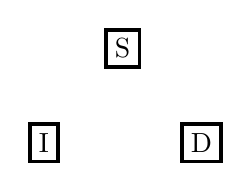
\begin{tikzpicture}
        \path (0,0)  node[RectObject] (x) {{\red S}}; 
        \path (1.,-1.2) node[RectObject] (y) {D};
        \path (-1,-1.2)  node[RectObject] (z) {I};
      \end{tikzpicture}
    \end{flushleft}
  \vspace{-1cm}
 \plot{image-v-init}{width=\textwidth}{}
\end{frame}



\begin{frame}
  \vspace{.63cm}
    \begin{flushleft}
      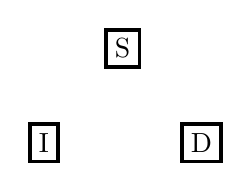
\begin{tikzpicture}
        \path (0,0)  node[RectObject] (x) {S}; 
        \path (1.,-1.2) node[RectObject] (y) {D};
        \path (-1,-1.2)  node[RectObject] (z) {{\red I}};
      \end{tikzpicture}
    \end{flushleft}
  \vspace{-1cm}
 \plot{image-v-tomo}{width=\textwidth}{}
\end{frame}

\begin{frame}
  \vspace{.63cm}
    \begin{flushleft}
      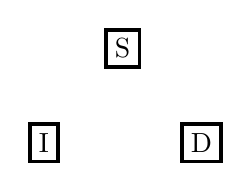
\begin{tikzpicture}
        \path (0,0)  node[RectObject] (x) {S}; 
        \path (1.,-1.2) node[RectObject] (y) {{\red D}};
        \path (-1,-1.2)  node[RectObject] (z) {I};
      \end{tikzpicture}
    \end{flushleft}
  \vspace{-1cm}
 \plot{image-vel_fwi_May_e}{width=\textwidth}{}
\end{frame}



\begin{frame}
  \vspace{.63cm}
    \begin{flushleft}
      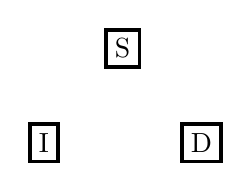
\begin{tikzpicture}
        \path (0,0)  node[RectObject] (x) {{\red S}}; 
        \path (1.,-1.2) node[RectObject] (y) {D};
        \path (-1,-1.2)  node[RectObject] (z) {I};
      \end{tikzpicture}
    \end{flushleft}
  \vspace{-1cm}
  \begin{columns}
    \column{0.5\textwidth}
      \plot{cip-v-init-00}{width=0.8\textwidth}{}
    \column{0.5\textwidth}
      \plot{cip-v-init-01}{width=0.8\textwidth}{}
  \end{columns}
\end{frame}



\begin{frame}
  \vspace{.63cm}
    \begin{flushleft}
      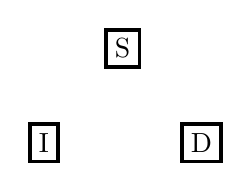
\begin{tikzpicture}
        \path (0,0)  node[RectObject] (x) {S}; 
        \path (1.,-1.2) node[RectObject] (y) {D};
        \path (-1,-1.2)  node[RectObject] (z) {{\red I}};
      \end{tikzpicture}
    \end{flushleft}
  \vspace{-1cm}
  \begin{columns}
    \column{0.5\textwidth}
      \plot{cip-v-tomo-00}{width=0.8\textwidth}{}
    \column{0.5\textwidth}
      \plot{cip-v-tomo-01}{width=0.8\textwidth}{}
  \end{columns}
\end{frame}




\begin{frame} \frametitle{PhD thesis}
  \Large

  \begin{enumerate}
  \setcounter{enumi}{1}    
    \item \gray{Cascaded wavefield tomography \& inversion using extended common image point gathers: a case study}
    \item Seismic tomography using local-correlation functions
    \item \gray{Imaging the model through wave equations }
    \item \gray{Extended imaging, deconvolution, and two-way wavefields: a comparison}
  \end{enumerate} 
\end{frame}


\inputdir{lcorr}




\begin{frame}
  \plot{f}{}{\klabel{10}{30}{${ f(t)}$}}
\end{frame}

\begin{frame}
  \plot{g}{}{\klabel{10}{30}{${ g(t)}$}}
\end{frame}

\begin{frame}
  \plot{corr}{}{\wlabel{20}{5}{$f\star g,\sigma=0.04$s}}
\end{frame}

\begin{frame}
  \plot{gcorr}{}
    {\wlabel{20}{5}{$f\star g,\sigma\rightarrow \infty$}}
\end{frame}

\inputdir{example}
\begin{frame}
  \plot{vel-neg}{}{\klabel{72}{30}{slow}}
\end{frame}

\begin{frame}
  \plot{vel-zer}{}{\klabel{72}{30}{correct}}
\end{frame}

\begin{frame}
  \plot{vel-pos}{}{\klabel{72}{30}{fast}}
\end{frame}

\begin{frame}
  \plot{data-comp}{}{}
\end{frame}

\begin{frame}
  \plot{gr-penaltyBP-local-vel-neg}{}
    {\klabel{15}{-3}{$\sigma=0.1s$}
     \klabel{70}{-3}{slow}
      }
\end{frame}
\begin{frame}
  \plot{gr-penaltyBP-local-vel-zer}{}
    {\klabel{15}{-3}{$\sigma=0.1s$}
     \klabel{70}{-3}{correct}
      }
\end{frame}
\begin{frame}
  \plot{gr-penaltyBP-local-vel-pos}{}
    {\klabel{15}{-3}{$\sigma=0.1s$}
     \klabel{70}{-3}{fast}
      }
\end{frame}
\begin{frame}
  \plot{gr-penaltyBP-global-vel-pos}{}
    {\klabel{15}{-3}{$\sigma\rightarrow \infty$}
     \klabel{70}{-3}{fast}
      }
\end{frame}



\begin{frame} \frametitle{PhD thesis}
  \Large

  \begin{enumerate}
  \setcounter{enumi}{1}    
    \item \gray{Cascaded wavefield tomography \& inversion using extended common image point gathers: a case study}
    \item \gray{Seismic tomography using local-correlation functions}
    \item Imaging the model through wave equations 
    \item \gray{Extended imaging, deconvolution, and two-way wavefields: a comparison}
  \end{enumerate} 
\end{frame}




\inputdir{XFig}



\begin{frame}
  \plot{f-3}{width=0.7\textwidth}{\klabellarge{45}{-5}{(after Singh et al., 2015)}}
\end{frame}

\begin{frame}
  \plot{f-2}{width=0.7\textwidth}{\klabellarge{45}{-5}{(after Singh et al., 2015)}}
\end{frame}

\begin{frame}
  \plot{f-1}{width=0.7\textwidth}{\klabellarge{45}{-5}{(after Singh et al., 2015)}}
\end{frame}

\begin{frame}
  \plot{f-0}{width=0.7\textwidth}{\klabellarge{45}{-5}{(after Singh et al., 2015)}}
\end{frame}

\begin{frame}
  \plot{g+1}{width=0.7\textwidth}{\klabellarge{45}{-5}{(after Singh et al., 2015)}}
\end{frame}

\begin{frame}
  \plot{g+2}{width=0.7\textwidth}{\klabellarge{45}{-5}{(after Singh et al., 2015)}}
\end{frame}






\inputdir{inversion_03}
\begin{frame}
  \plot{p-600-03}{}{}
\end{frame}


\begin{frame}
  \plot{p-600-03}{}{\wlabelh{25}{40}{{\Huge ?}}}
\end{frame}


\begin{frame}
  \plot{density2}{}{}
\end{frame}


\inputdir{.}
\begin{frame}
  \plot{manduca}{width=0.7\textwidth}{\klabel{25}{0}{{\Large (Manduca et al.,2001)}}}
\end{frame}





\begin{frame}
  \begin{align}
    \only<1-1>{ \partial_t^2 u(\xx,\xs,t) s^2(\xx) = \nabla^2 u(\xx,\xs,t)  \white {\underbrace{\partial_t^2}_{\text{$\bf A$}}}} \nonumber
    \only<2-2>{\underbrace{\partial_t^2 u(\xx,\xs,t) }_{\text{$\bf A$}} s^2(\xx) = \nabla^2 u(\xx,\xs,t)\white {\underbrace{\partial_t^2}_{\text{$\bf A$}}}} \nonumber
    \only<3-3>{\underbrace{\partial_t^2 u(\xx,\xs,t) }_{\text{$\bf A$}} \underbrace{s^2(\xx)}_{\text{$\bf m$}} = \nabla^2 u(\xx,\xs,t) \white {\underbrace{\partial_t^2}_{\text{$\bf A$}}}} \nonumber
    \only<4-4>{\underbrace{\partial_t^2 u(\xx,\xs,t) }_{\text{$\bf A$}} \underbrace{s^2(\xx)}_{\text{$\bf m$}} = \underbrace{\nabla^2 u(\xx,\xs,t)}_{\text{$\bf b$}} \white {\underbrace{\partial_t^2}_{\text{$\bf A$}}}} \nonumber
  \end{align}
\sep

$s$: slowness 
\end{frame}

\begin{frame}
  \[
    J(\m) = \ltnorm{{\bf A}{\bf m} -{\bf b}}
  \]
\end{frame}

\begin{frame}
  \begin{columns}
    \column{0.5\textwidth}
      \[
        s^2 = \dfrac {\sum\limits_{t,\xs} \partial_t^2 u  \nabla^2 u}{ \sum\limits_{t,\xs} \lp\partial_t^2 u\rp^2}
      \]
    \column{0.5\textwidth}
  \end{columns}
\end{frame}

\begin{frame}
  \begin{columns}
    \column{0.5\textwidth}
      \[
         s^2 = \dfrac {\sum\limits_{t,\xs} \partial_t^2 u  \nabla^2 u}{ \sum\limits_{t,\xs} \lp\partial_t^2 u\rp^2}
      \]
    \column{0.5\textwidth}
      \[
        I = \dfrac {\sum\limits_{t,\xs}  u_s  u_r}{ \sum\limits_{t,\xs} \lp u_s\rp^2}
      \]
  \end{columns}
\end{frame}


\inputdir{inversion_01}

\begin{frame}
  \plot{pasurf_cpbox}{}{}
\end{frame}


\begin{frame}
  \plot{vbox}{width=0.8\textwidth}{\klabel{35}{-4}{input model}}
\end{frame}
\begin{frame}
  \plot{p-600-01}{width=0.8\textwidth}{\klabel{35}{-4}{retrieved wavefield}}
\end{frame}

\begin{frame}
  \plot{s2-01}{width=0.8\textwidth}{\klabel{35}{-4}{inverted model}}
\end{frame}


\inputdir{inversion_02}


\begin{frame}
  \plot{vbox}{width=0.8\textwidth}{\klabel{35}{-4}{smooth model}}
\end{frame}
\begin{frame}
  \plot{p-600-02}{width=0.8\textwidth}{\klabel{35}{-4}{retrieved wavefield}}
\end{frame}
\begin{frame}
  \plot{s2-01}{width=0.8\textwidth}{\klabel{35}{-4}{inverted model}}
\end{frame}










\begin{frame}
  \begin{align}
    \only<1-1>{   \partial_z u(\xx,\xs,t) \dfrac{1}{\rho(\xx)} = -\partial_t v_z \lp \xx,\xs,t \rp  } \nonumber
    \only<2-2>{\underbrace{\partial_z u(\xx,\xs,t) }_{\text{$\bf A$}} \dfrac{1}{\rho(\xx)} = -\partial_t v_z \lp \xx,\xs,t \rp} \nonumber
    \only<3-3>{\underbrace{\partial_z u(\xx,\xs,t) }_{\text{$\bf A$}} \underbrace{\dfrac{1}{\rho(\xx)}}_{\text{$\m$}} = -\partial_t v_z \lp \xx,\xs,t \rp} \nonumber
    \only<4-4>{\underbrace{\partial_z u(\xx,\xs,t) }_{\text{$\bf A$}} \underbrace{\dfrac{1}{\rho(\xx)}}_{\text{$\m$}} = \underbrace{-\partial_t v_z \lp \xx,\xs,t \rp}_{\text{$\bf b$}}} \nonumber
  \end{align}
\sep

$v_z$: particle velocity

$u$: pressure
\end{frame} 

\begin{frame}
  \[
    J(\m) = \ltnorm{{\bf A}{\bf m} -{\bf b}}
  \]
\sep
$v_z$: particle velocity 

$u$: pressure 

\end{frame} 


\begin{frame}
  \[
    \dfrac{1}{\rho}  = \dfrac{\sum\limits_{t,\xx_s}  \partial_t V_z \partial_z u }{ \sum\limits_{t,\xx_s} \lp \partial_z u \rp^2}
  \]

\end{frame}

\inputdir{inversion_04}

\begin{frame}
  \plot{vbox-04}{width=0.8\textwidth}{\klabel{35}{-4}{input model}}
\end{frame}

\begin{frame}
  \plot{p-600-04}{width=0.8\textwidth}{\klabel{35}{-4}{retrieved wavefield}}
\end{frame}

\begin{frame}
  \plot{density2-04}{width=0.8\textwidth}{\klabel{35}{-4}{inverted model}}
\end{frame}

\inputdir{inversion_03}
\begin{frame}
  \plot{density2-03}{width=0.8\textwidth}{\klabel{35}{-4}{inverted model}}
\end{frame}










\begin{frame} \frametitle{PhD thesis}
  \Large

  \begin{enumerate}
  \setcounter{enumi}{1}    
    \item \gray{Cascaded wavefield tomography \& inversion using extended common image point gathers: a case study}
    \item \gray{Seismic tomography using local-correlation functions}
    \item \gray{Imaging the model through wave equations }
    \item Extended imaging, deconvolution, and two-way wavefields: a comparison
  \end{enumerate} 
\end{frame}







\begin{frame}
  \[
     R(\xx,\hh,\tau) =
     \sum_{t} u_s(\xx+\hh,t+\tau) u_r(\xx-\hh,t-\tau)
  \]
\sep  
  \itab{$u_s$: source wavefield} \\ 
  \itab{$u_r$: receiver wavefield}\\
  \itab{$\hh,\tau$: space and time-lags}  
\end{frame}





\begin{frame} \frametitle{ extended imaging}
 \[
  R = { U_s}^\top{u_r}
\]
\sep

${ U_s}^\top$: extended imaging 

$\UR$: receiver  wavefield
\end{frame} 

\begin{frame} \frametitle{deconvolution extended imaging}
 \[
  { U_s} R \approx {u_r}
\]
\sep

${ U_s}$: adjoint of extended imaging 

$\UR$: receiver wavefield
\end{frame} 

\begin{frame} \frametitle{deconvolution extended imaging}
\[
  \lp { U_s}^\top{ U_s} +\epsilon^2 {\bf I}\rp R = {U_s}^\top {u_r}
\]
\sep
$R$: extended deconvolution image
\end{frame} 







\inputdir{wavefields_00}

\begin{frame}
  \plot{ro}{}{}
\end{frame}


\begin{frame}
  \plot{data}{}{}
\end{frame}



\begin{frame} \frametitle{extended correlation\hfill RTM}
  \vspace{-0.5cm}
  \begin{columns}
    \column{0.33\textwidth}
      \plot{01_eimg_Con-090}{height=0.7\textheight}{\klabel{10}{-10}{slow}}
    \column{0.33\textwidth}
      \plot{01_eimg_Con-100}{height=0.7\textheight}{\klabel{0}{-10}{correct}}
    \column{0.33\textwidth}
      \plot{01_eimg_Con-110}{height=0.7\textheight}{\klabel{10}{-10}{fast}}
  \end{columns}
\end{frame}


\begin{frame} \frametitle{extended correlation\hfill Marchenko}
  \vspace{-.5cm}
  \begin{columns}
    \column{0.33\textwidth}
      \plot{00_eimg_Mar-090}{height=0.7\textheight}{\klabel{10}{-10}{slow}}
    \column{0.33\textwidth}
      \plot{00_eimg_Mar-100}{height=0.7\textheight}{\klabel{0}{-10}{correct}}
    \column{0.33\textwidth}
      \plot{00_eimg_Mar-110}{height=0.7\textheight}{\klabel{10}{-10}{fast}}
  \end{columns}
\end{frame}


\begin{frame} \frametitle{extended deconvolution\hfill Marchenko}
  \vspace{-.5cm}
  \begin{columns}
    \column{0.33\textwidth}
      \plot{00_eimg_Mar-090_dec}{height=0.7\textheight}{\klabel{10}{-10}{slow}}
    \column{0.33\textwidth}
      \plot{00_eimg_Mar-100_dec}{height=0.7\textheight}{\klabel{0}{-10}{correct}}
    \column{0.33\textwidth}
      \plot{00_eimg_Mar-110_dec}{height=0.7\textheight}{\klabel{10}{-10}{fast}}
  \end{columns}
\end{frame}







\inputdir{extended_imaging}

\begin{frame}\frametitle{velocity model}
  \plot{vel}{width=0.9\textwidth}{}
\end{frame}

\begin{frame}  \frametitle{extended images, slow model\hfill }
  \plot{section_xgathers-090}{width=0.9\textwidth}{}
\end{frame}

\begin{frame} \frametitle{extended images, correct model \hfill }
  \plot{section_xgathers-100}{width=0.9\textwidth}{}
\end{frame}

\begin{frame} \frametitle{extended images, fast model\hfill }
  \plot{section_xgathers-110}{width=0.9\textwidth}{}
\end{frame}


\inputdir{gom}
\begin{frame}
  \big{Gulf of Mexico dataset}
\end{frame}
\begin{frame}\frametitle{ Gulf of Mexico velocity model }
 \plot{vel}{width=0.9\textwidth}{}
\end{frame}

\begin{frame}\frametitle{initial image \hfill RTM }
  \plot{img_xgathers_init_RTM}{width=0.9\textwidth}{}
\end{frame}

\begin{frame}\frametitle{extended RTM images  \hfill correlation }
  \plot{section_xgathers_init_RTM}{width=0.9\textwidth}{}
\end{frame}

\begin{frame}\frametitle{extended RTM images  \hfill deconvolution }
  \plot{section_xgathers_RTM}{width=0.9\textwidth}{}
\end{frame}


\begin{frame}\frametitle{initial image \hfill Marchenko }
  \plot{img_xgathers_init_Mar}{width=0.9\textwidth}{}
\end{frame}

\begin{frame}\frametitle{extended Marchenko images  \hfill correlation }
  \plot{section_xgathers_init_Mar}{width=0.9\textwidth}{}
\end{frame}

\begin{frame}\frametitle{extended Marchenko images  \hfill deconvolution }
  \plot{section_xgathers_Mar}{width=0.9\textwidth}{}
\end{frame}

\begin{frame}\frametitle{deconvolved image \hfill Marchenko }
  \plot{img_xgathers_Mar}{width=0.9\textwidth}{}
\end{frame}
\begin{frame}\frametitle{initial image \hfill Marchenko }
  \plot{img_xgathers_init_Mar}{width=0.9\textwidth}{}
\end{frame}
\begin{frame}\frametitle{deconvolved image \hfill Marchenko }
  \plot{img_xgathers_Mar}{width=0.9\textwidth}{}
\end{frame}
\begin{frame}\frametitle{deconvolved image \hfill RTM }
  \plot{img_xgathers_RTM}{width=0.9\textwidth}{}
\end{frame}



\begin{frame}\frametitle{acknowledgments}
\Large
\begin{itemize}

\item {Paul Sava}\\
\item {Dave Hale, Yaoguo Li, Luis Tenorio, and Kamini Singha}\\
\item { Roel Snieder, Ilya Tsvankin, Gerhard Pratt, Bruce VerWest, Tariq Alkhalifah, and Antoine Guitton}\\
\item {Satyan Singh,Yuting Duan, Nishant Kamath, and Vladimir Li} 
\item {Diane, Shingo, Pam, Dawn, and Michelle}
\end{itemize}
\end{frame}

\inputdir{.}

\begin{frame}\frametitle{acknowledgments}
\plot{Carla_retrato-32}{height=0.8\textheight}{}
\end{frame}

\begin{frame}\frametitle{acknowledgments}
\plot{foto}{height=0.8\textheight}{}
\end{frame}



\begin{frame}
\end{frame}





